%%%%%%%%%%%%%%%%%%%%%%%%%%%%%%%%%%%%%%%%%%%%%%%%%%%%%%%%%%%%%%%%%%%%%%%%%%%%%%%%%%%%%%%%%%%%%%%%%%%
%%%%%%%%%%%%%%%%%%%%%%%%%%%%%%%%%%%%%%%%%%%%%%%%%%%%%%%%%%%%%%%%%%%%%%%%%%%%%%%%%%%%%%%%%%%%%%%%%%%
%%%%%%%%%%%%%%%%%%%%%%%%%%%%%%%%%%%%%%%%%%%%%%%%%%%%%%%%%%%%%%%%%%%%%%%%%%%%%%%%%%%%%%%%%%%%%%%%%%%
%%%%%%%%%%%%%%%%%%%%%%%%%%%%%%%%%%%%%%%%%%%%%%%%%%%%%%%%%%%%%%%%%%%%%%%%%%%%%%%%%%%%%%%%%%%%%%%%%%%
\documentclass{beamer}
\usepackage[utf8]{inputenc}
\usepackage[spanish]{babel}
\decimalpoint
\usepackage{amsmath}
\usepackage{amsfonts}
\usepackage{amssymb}
\usepackage{graphicx}

\usepackage{bibentry}

\usepackage{movie15}

\usepackage{verbatim}
%\usepackage{authblk}

\usepackage{listings}
\usepackage{color}

% para la bibliografia
\usepackage[style=verbose,backend=bibtex]{biblatex}

\bibstyle{abbrv}

%%%%%%%%%%%%%%%%%%%%%%%%%%%%%%%%%%%%%%%%%%%%%%%%%%%%%%%%%%%%%%%%%%%%%%%%%%%%%%%%%%%%%%%%%%%%%%%%%%%
%%%%%%%%%%%%%%%%%%%%%%%%%%%%%%%%%%%%%%%%%%%%%%%%%%%%%%%%%%%%%%%%%%%%%%%%%%%%%%%%%%%%%%%%%%%%%%%%%%%

\addbibresource{referencias_estacionariedad.bib}
\addbibresource{referencias_fisiologia.bib}
\addbibresource{referencias_otros.bib}
\addbibresource{referencias_mixto.bib}

%%%%%%%%%%%%%%%%%%%%%%%%%%%%%%%%%%%%%%%%%%%%%%%%%%%%%%%%%%%%%%%%%%%%%%%%%%%%%%%%%%%%%%%%%%%%%%%%%%%
%%%%%%%%%%%%%%%%%%%%%%%%%%%%%%%%%%%%%%%%%%%%%%%%%%%%%%%%%%%%%%%%%%%%%%%%%%%%%%%%%%%%%%%%%%%%%%%%%%%

%\usetheme{Luebeck}
\usetheme{CambridgeUS}
\usecolortheme{beaver}
{
%\usetheme{Luebeck}
%\setbeamercolor{palette secondary}{use=structure,fg=white,bg=red}
%\setbeamercolor{palette tertiary}{use=structure,fg=white,bg=green}
}

%
%
%
\definecolor{rojo}{rgb}{0.62353,0.10588,0.13725}
\definecolor{rojo2}{rgb}{0.32353,0.050588,0.06725}
\definecolor{naranja}{rgb}{0.91765,0.23137,0.16078}
\definecolor{rosa}{rgb}{0.95294,0.53333,0.32157}
\definecolor{cafe}{rgb}{0.48627,0.14118,0.10196}
\definecolor{cafe2}{rgb}{0.243135,0.07059,0.05098}
\definecolor{cafe3}{rgb}{0.1215675,0.035295,0.02549}

\definecolor{gris}{gray}{0.925}
\definecolor{gris2}{gray}{0.8}

\definecolor{UniBlue}{RGB}{83,121,170}
\setbeamercolor{title}{fg=white,bg=rojo}
\setbeamercolor{frametitle}{fg=white,bg=rojo}
\setbeamercolor{structure}{fg=rojo,bg=gris2}

\setbeamercolor{alerted text}{fg=rojo,bg=cafe2}
%\setbeamercolor{alerted text}{bg=cafe3,fg=white}

\setbeamercolor{palette primary}{bg=rojo2,fg=white}
%\setbeamercolor{palette secondary}{bg=cafe3,fg=white}
\setbeamercolor{palette tertiary}{bg=cafe2,fg=white}
\setbeamercolor{palette quaternary}{use=structure,bg=naranja,fg=white}
\setbeamercolor{itemize item}{bg=naranja,fg=naranja}
\setbeamercolor{section number projected }{bg=rosa,fg=white}

\setbeamertemplate{itemize item}{\color{naranja}$\bullet$}

%%%%%%%%%%%%%%%%%%%%%%%%%%%%%%%%%%%%%%%%%%%%%%%%%%%%%%%%%%%%%%%%%%%%%%%%%%%%%%%%%%%%%%%%%%%%%%%%%%%
%%%%%%%%%%%%%%%%%%%%%%%%%%%%%%%%%%%%%%%%%%%%%%%%%%%%%%%%%%%%%%%%%%%%%%%%%%%%%%%%%%%%%%%%%%%%%%%%%%%

%\DeclareUnicodeCharacter{00A0}{ }

\lstset{ %
%  language=R,                     % the language of the code
  basicstyle=\footnotesize,       % the size of the fonts that are used for the code
}

%%%%%%%%%%%%%%%%%%%%%%%%%%%%%%%%%%%%%%%%%%%%%%%%%%%%%%%%%%%%%%%%%%%%%%%%%%%%%%%%%%%%%%%%%%%%%%%%%%%
%%%%%%%%%%%%%%%%%%%%%%%%%%%%%%%%%%%%%%%%%%%%%%%%%%%%%%%%%%%%%%%%%%%%%%%%%%%%%%%%%%%%%%%%%%%%%%%%%%%

\newtheorem{defn}{Definici\'on}
\newtheorem{thrm}{Teorema}
\newtheorem{demostracion}{Demostraci\'on}

\newcommand{\R}{\mathbb{R}}
%\newcommand{\el2}{L^2}
\newcommand{\intR}{\int_{-\infty}^{\infty}}
\newcommand{\intZ}{\int_{-\infty}^{0}}
\newcommand{\intPI}{\int_{-\pi}^{\pi}}
\newcommand{\simint}[1]{\int_{- #1 }^{ #1 }}
\newcommand{\prima}{^{\prime}}

\newcommand{\ddd}{$\delta$}

\newcommand{\aste}[1]{\widehat{ #1 }^{\star}}
\newcommand{\est}[1]{\widehat{ #1 }}

\newcommand{\COS}[1]{\mathrm{cos}\left( #1 \right)}
\newcommand{\SEN}[1]{\mathrm{sen}\left( #1 \right)}

\newcommand{\E}[1]{\mathrm{E}\left[ #1 \right]}
\newcommand{\Var}[1]{\mathrm{Var}\left( #1 \right)}
\newcommand{\Cov}[1]{\mathrm{Cov}\left( #1 \right)}
\newcommand{\abso}[1]{\left| #1 \right|}

%%%%%%%%%%%%%%%%%%%%%%%%%%%%%%%%%%%%%%%%%%%%%%%%%%%%%%%%%%%%%%%%%%%%%%%%%%%%%%%%%%%%%%%%%%%%%%%%%%%
%%%%%%%%%%%%%%%%%%%%%%%%%%%%%%%%%%%%%%%%%%%%%%%%%%%%%%%%%%%%%%%%%%%%%%%%%%%%%%%%%%%%%%%%%%%%%%%%%%%

\title[Estacionariedad en PSG de adultos mayores]
{Estacionariedad d\'ebil en registros de polisomnogr\'aficaos de adultos mayores,
como posible marcador de deterioro cognitivo}

\author[Enciso Alva]
{Julio Cesar Enciso Alva}

\institute[LIMA]
{Licenciatura en Matem\'aticas Aplicadas}

\date[Mayo 2017]
{Seminario de investigaci\'on\\ Mayo de 2017}

\titlegraphic{
\hspace*{8cm}~
\includegraphics[width=9em]{./material1/SIGLAS_UAEH_02.png}
}

%%%%%%%%%%%%%%%%%%%%%%%%%%%%%%%%%%%%%%%%%%%%%%%%%%%%%%%%%%%%%%%%%%%%%%%%%%%%%%%%%%%%%%%%%%%%%%%%%%%
%%%%%%%%%%%%%%%%%%%%%%%%%%%%%%%%%%%%%%%%%%%%%%%%%%%%%%%%%%%%%%%%%%%%%%%%%%%%%%%%%%%%%%%%%%%%%%%%%%%
%%%%%%%%%%%%%%%%%%%%%%%%%%%%%%%%%%%%%%%%%%%%%%%%%%%%%%%%%%%%%%%%%%%%%%%%%%%%%%%%%%%%%%%%%%%%%%%%%%%
%%%%%%%%%%%%%%%%%%%%%%%%%%%%%%%%%%%%%%%%%%%%%%%%%%%%%%%%%%%%%%%%%%%%%%%%%%%%%%%%%%%%%%%%%%%%%%%%%%%

%%%%%%%%%%%%%%%%%%%%%%%%%%%%%%%%%%%%%%%%%%%%%%%%%%%%%%%%%%%%%%%%%%%%%%%%%%%%%%%%%%%%%%%%%%%%%%%%%%%
%%%%%%%%%%%%%%%%%%%%%%%%%%%%%%%%%%%%%%%%%%%%%%%%%%%%%%%%%%%%%%%%%%%%%%%%%%%%%%%%%%%%%%%%%%%%%%%%%%%

\begin{document}

\frame{\titlepage}

\begin{frame}
\tableofcontents
\end{frame}

%%%%%%%%%%%%%%%%%%%%%%%%%%%%%%%%%%%%%%%%%%%%%%%%%%%%%%%%%%%%%%%%%%%%%%%%%%%%%%%%%%%%%%%%%%%%%%%%%%%
%%%%%%%%%%%%%%%%%%%%%%%%%%%%%%%%%%%%%%%%%%%%%%%%%%%%%%%%%%%%%%%%%%%%%%%%%%%%%%%%%%%%%%%%%%%%%%%%%%%
%%%%%%%%%%%%%%%%%%%%%%%%%%%%%%%%%%%%%%%%%%%%%%%%%%%%%%%%%%%%%%%%%%%%%%%%%%%%%%%%%%%%%%%%%%%%%%%%%%%

\section{Introducci\'on}

%%%%%%%%%%%%%%%%%%%%%%%%%%%%%%%%%%%%%%%%%%%%%%%%%%%%%%%%%%%%%%%%%%%%%%%%%%%%%%%%%%%%%%%%%%%%%%%%%%%
%%%%%%%%%%%%%%%%%%%%%%%%%%%%%%%%%%%%%%%%%%%%%%%%%%%%%%%%%%%%%%%%%%%%%%%%%%%%%%%%%%%%%%%%%%%%%%%%%%%

\subsection{Antecedentes}

\begin{frame}\frametitle{Antecedentes}
\begin{itemize}
\item Encuesta Intercensal 2015 (INEGI): 12,500,000 adultos mayores, 10.4 \%  de la 
poblaci\'on \cite{Intercensal15}

\item Posible relaci\'on trastornos del sue\~no y DC en la vejez
\cite{Amer13,Miyata13,Potvin12}

\item Epidemiolog\'ia del DC en Hidalgo: eficiencia del sue\~no\cite{VazquezTagle16}

\item DFA en registros de PSG \cite{Valeria}: exponente de Hurst diferente en sujetos 
con y sin DC 

\item Se buscan marcadores cl\'inicos para el diagn\'ostico de DC
\end{itemize}
\end{frame}

%%%%%%%%%%%%%%%%%%%%%%%%%%%%%%%%%%%%%%%%%%%%%%%%%%%%%%%%%%%%%%%%%%%%%%%%%%%%%%%%%%%%%%%%%%%%%%%%%%%
%%%%%%%%%%%%%%%%%%%%%%%%%%%%%%%%%%%%%%%%%%%%%%%%%%%%%%%%%%%%%%%%%%%%%%%%%%%%%%%%%%%%%%%%%%%%%%%%%%%

\subsection{Objetivos}

\begin{frame}\frametitle{Pregunta de investigaci\'on}
\textbf{
¿Es posible que la caracterizaci\'on de registros de PSG como series de tiempo d\'ebilmente 
estacionarias, pueda ser usada como un marcador en el diagn\'ostico cl\'inico de PDC en adultos 
mayores?
}

\end{frame}

%%%%%%%%%%%%%%%%%%%%%%%%%%%%%%%%%%%%%%%%%%%%%%%%%
%%%%%%%%%%%%%%%%%%%%%%%%%%%%%%%%%%%%%%%%%%%%%%%%%

\begin{frame}\frametitle{Objetivos}
{\small
\begin{description}
%\textbf{General.} 
\item[General:]
Detectar, a partir de pruebas formales, las presencia de estacionariedad d\'ebil 
en registros de PSG para adultos mayores% con y sin PDC

%\textbf{Espec\'ificos} 
\item[Espec\'ificos:]
\end{description}
\begin{itemize}
\item Estudiar la definici\'on de estacionariedad y sus consecuencias en un modelo

\item Investigar c\'omo detectar si una serie de tiempo dada proviene de un proceso
d\'ebilmente estacionario

\item Usando los an\'alisis hallados, determinar si los datos considerados provienen de 
procesos débilmente estacionarios.
Revisar si esta informaci\'on muestra diferencias entre sujetos con y sin PDC
\end{itemize}
}
\end{frame}

%%%%%%%%%%%%%%%%%%%%%%%%%%%%%%%%%%%%%%%%%%%%%%%%%%%%%%%%%%%%%%%%%%%%%%%%%%%%%%%%%%%%%%%%%%%%%%%%%%%
%%%%%%%%%%%%%%%%%%%%%%%%%%%%%%%%%%%%%%%%%%%%%%%%%%%%%%%%%%%%%%%%%%%%%%%%%%%%%%%%%%%%%%%%%%%%%%%%%%%
%%%%%%%%%%%%%%%%%%%%%%%%%%%%%%%%%%%%%%%%%%%%%%%%%%%%%%%%%%%%%%%%%%%%%%%%%%%%%%%%%%%%%%%%%%%%%%%%%%%

\section{Conceptos}

%%%%%%%%%%%%%%%%%%%%%%%%%%%%%%%%%%%%%%%%%%%%%%%%%%%%%%%%%%%%%%%%%%%%%%%%%%%%%%%%%%%%%%%%%%%%%%%%%%%
%%%%%%%%%%%%%%%%%%%%%%%%%%%%%%%%%%%%%%%%%%%%%%%%%%%%%%%%%%%%%%%%%%%%%%%%%%%%%%%%%%%%%%%%%%%%%%%%%%%

\subsection{Fisiolog\'ia}

\begin{frame}\frametitle{Conceptos}
\begin{description}
\item[Adulto Mayor.] Individuo de 60 a\~nos o m\'as \cite{Hita14}.

\item[Deterioro cognitivo leve\footnote{Usado como posible deterioro cognitivo (PDC)}.] 
%\item[Deterioro cognitivo leve.] 
Alteraci\'on adquirida y prolongada de funciones cognitivas; no s\'indrome focal, no demencia 
\cite{Robles02}
%\end{description}
%\end{frame}
%
%\begin{frame}
%\begin{description}
\item[Sue\~no.] Proceso vital c\'iclico complejo y activo; caracter\'isticas\cite{CarrilloMora}:
\begin{itemize}
\item Disminuci\'on de conciencia y reactividad
\item F\'acilmente reversible
\item Inmovilidad muscular
\item Periodicidad circadiana
\item Postura estereotipada
\item La privaci\'on induce alteraciones
\end{itemize}
\end{description}
\end{frame}

%%%%%%%%%%%%%%%%%%%%%%%%%%%%%%%%%%%%%%%%%%%%%%%%%
%%%%%%%%%%%%%%%%%%%%%%%%%%%%%%%%%%%%%%%%%%%%%%%%%

\begin{frame}\frametitle{Conceptos}
\begin{description}
\item[Electroencefalograma.] Registro de las fluctuaciones en potenciales el\'ectricos en el 
cerebro
\end{description}
\begin{figure}
\centering
\includegraphics[width=0.6\linewidth]{Fig.png} 
\caption{Sistema de referencia 10--20, recomendado por la
International Federation of EEG Societies
}
\label{img1020}
\end{figure}
\end{frame}

%%%%%%%%%%%%%%%%%%%%%%%%%%%%%%%%%%%%%%%%%%%%%%%%%%%%%%%%%%%%%%%%%%%%%%%%%%%%%%%%%%%%%%%%%%%%%%%%%%%
%%%%%%%%%%%%%%%%%%%%%%%%%%%%%%%%%%%%%%%%%%%%%%%%%%%%%%%%%%%%%%%%%%%%%%%%%%%%%%%%%%%%%%%%%%%%%%%%%%%

\subsection{Matem\'aticas}

\begin{frame}\frametitle{Conceptos}
\begin{defn}[Proceso estoc\'astico]
Un proceso estoc\'astico $\{ X(t) \}$ es una familia de variables aleatorias en los reales, 
indexadas por $t \in T \subseteq \R$.
%\label{proc_estocastico}
\end{defn}

\begin{defn}[Estacionariedad d\'ebil]
Se dice de un proceso $\{ X(t) \}$ si para cualesquiera tiempos 
admisibles $t, s, t+\tau, s+\tau$ se cumple
\begin{itemize}
\item $\E{X(t)} = \E{X(t+\tau)}$
\item $\E{X(t)X(s)} = \E{X(t+\tau)X(s+\tau)}$
\end{itemize}
\end{defn}
\end{frame}

%%%%%%%%%%%%%%%%%%%%%%%%%%%%%%%%%%%%%%%%%%%%%%%%%
%%%%%%%%%%%%%%%%%%%%%%%%%%%%%%%%%%%%%%%%%%%%%%%%%

%\begin{frame}%\frametitle{}
%
%\end{frame}

%%%%%%%%%%%%%%%%%%%%%%%%%%%%%%%%%%%%%%%%%%%%%%%%%
%%%%%%%%%%%%%%%%%%%%%%%%%%%%%%%%%%%%%%%%%%%%%%%%%

%\begin{frame}%\frametitle{}
%
%\end{frame}

%%%%%%%%%%%%%%%%%%%%%%%%%%%%%%%%%%%%%%%%%%%%%%%%%%%%%%%%%%%%%%%%%%%%%%%%%%%%%%%%%%%%%%%%%%%%%%%%%%%
%%%%%%%%%%%%%%%%%%%%%%%%%%%%%%%%%%%%%%%%%%%%%%%%%%%%%%%%%%%%%%%%%%%%%%%%%%%%%%%%%%%%%%%%%%%%%%%%%%%

\section{Metodolog\'ia}

%%%%%%%%%%%%%%%%%%%%%%%%%%%%%%%%%%%%%%%%%%%%%%%%%%%%%%%%%%%%%%%%%%%%%%%%%%%%%%%%%%%%%%%%%%%%%%%%%%%
%%%%%%%%%%%%%%%%%%%%%%%%%%%%%%%%%%%%%%%%%%%%%%%%%%%%%%%%%%%%%%%%%%%%%%%%%%%%%%%%%%%%%%%%%%%%%%%%%%%

\section{Resultados}

\begin{frame}\frametitle{Resultados principales}
\begin{itemize}
\item Cada \'epoca fue clasificada 'posiblemente estacionaria' (PE) no se rechaza la 
hip\'otesis de estacionariedad ($\alpha < 0.05$) en PSR

\item Debido a la variabilidad entre sujetos, se consider\'o la proporci\'on de \'epocas PE
en cada etapa
\begin{equation*}
\text{\% \'epocas PE} = \frac{\text{\# \'epocas PE en MOR}}{\text{\# \'epocas en MOR}}
\end{equation*}

\item Las proporciones se compararon:
\begin{itemize}
\item MOR vs NMOR (individual y grupal)
\item Grupo Control vs Grupo PDC (en cada etapa de sue\~no)
\end{itemize}
\end{itemize}
\end{frame}

%%%%%%%%%%%%%%%%%%%%%%%%%%%%%%%%%%%%%%%%%%%%%%%%%
%%%%%%%%%%%%%%%%%%%%%%%%%%%%%%%%%%%%%%%%%%%%%%%%%

\begin{frame}\frametitle{MOR vs NMOR, individual}
\begin{figure}
\centering
\begin{tabular}{c}
\begin{tabular}{ccccc}
\includegraphics[width=0.15\textwidth]{./cabecitas/cabecita_VCR.pdf} &
\includegraphics[width=0.15\textwidth]{./cabecitas/cabecita_MJH.pdf} &
\includegraphics[width=0.15\textwidth]{./cabecitas/cabecita_JAE.pdf} &
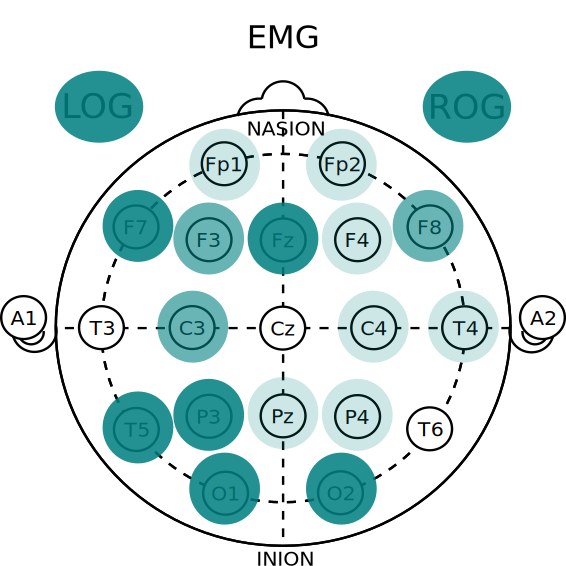
\includegraphics[width=0.15\textwidth]{./cabecitas/cabecita_GHA.pdf} &
\includegraphics[width=0.15\textwidth]{./cabecitas/cabecita_MFGR.pdf} \\
VCR & MJH & JAE & GHA & MFGR
\end{tabular}
\\
\begin{tabular}{cccc}
\includegraphics[width=0.15\textwidth]{./cabecitas/cabecita_CLO.pdf} &
\includegraphics[width=0.15\textwidth]{./cabecitas/cabecita_RLO.pdf} &
\includegraphics[width=0.15\textwidth]{./cabecitas/cabecita_RRU.pdf} &
\includegraphics[width=0.15\textwidth]{./cabecitas/cabecita_JGZ.pdf} \\
CLO & RLO & RRU & JGZ
\end{tabular}
\end{tabular}
\caption{En azul las zonas donde se encontraron diferencias significativas}
%\label{cabecitas_munchas}
\end{figure}
\end{frame}

%%%%%%%%%%%%%%%%%%%%%%%%%%%%%%%%%%%%%%%%%%%%%%%%%
%%%%%%%%%%%%%%%%%%%%%%%%%%%%%%%%%%%%%%%%%%%%%%%%%

\begin{frame}\frametitle{Gpo. Control vs Gpo. PDC}
\begin{figure}
\centering
\begin{tabular}{rl}
{\Large \textbf{MOR}}
&
\includegraphics[width=0.6\linewidth]
{./new170424/Comparacion_gpos_MOR.pdf} 
\\
{\Large \textbf{NMOR}}
&
\includegraphics[width=0.6\linewidth]
{./new170424/Comparacion_gpos_NMOR.pdf} 
\end{tabular}
\caption{ Promedio $\pm$ 1 desviac\'on est\'andar. Control: azul, PDC: rojo.}
\end{figure}
\end{frame}

%%%%%%%%%%%%%%%%%%%%%%%%%%%%%%%%%%%%%%%%%%%%%%%%%
%%%%%%%%%%%%%%%%%%%%%%%%%%%%%%%%%%%%%%%%%%%%%%%%%

\begin{frame}\frametitle{MOR vs NMOR, grupal}
\begin{figure}
\centering
\begin{tabular}{rl}
{\Large \textbf{Gpo. Control}}
&
\includegraphics[width=0.6\linewidth]
{./new170424/comp_etapas_gpos_NORMALMOR_vs_NMOR.pdf} 
\\
{\Large \textbf{Gpo. PDC}}
&
\includegraphics[width=0.6\linewidth]
{./new170424/comp_etapas_gpos_PDCMOR_vs_NMOR.pdf} 
\end{tabular}
\caption{ Promedio $\pm$ 1 desviac\'on est\'andar. MOR: verde, NMOR: negro.}
\end{figure}
\end{frame}

%%%%%%%%%%%%%%%%%%%%%%%%%%%%%%%%%%%%%%%%%%%%%%%%%
%%%%%%%%%%%%%%%%%%%%%%%%%%%%%%%%%%%%%%%%%%%%%%%%%

\begin{frame}\frametitle{MOR vs NMOR, diferencias significativas}
\begin{figure}
\centering
\includegraphics[width=0.4\linewidth]
{cabecita.pdf} 
\caption{Sitios donde se encontraron diferencias 
significativas en la comparaci\'on entre el porcentaje de \'epocas PE durante sue\~no MOR y NMOR, 
para el grupo Control}
\end{figure}
\end{frame}

%%%%%%%%%%%%%%%%%%%%%%%%%%%%%%%%%%%%%%%%%%%%%%%%%
%%%%%%%%%%%%%%%%%%%%%%%%%%%%%%%%%%%%%%%%%%%%%%%%%

%\begin{frame}%\frametitle{}
%
%\end{frame}

%%%%%%%%%%%%%%%%%%%%%%%%%%%%%%%%%%%%%%%%%%%%%%%%%%%%%%%%%%%%%%%%%%%%%%%%%%%%%%%%%%%%%%%%%%%%%%%%%%%
%%%%%%%%%%%%%%%%%%%%%%%%%%%%%%%%%%%%%%%%%%%%%%%%%%%%%%%%%%%%%%%%%%%%%%%%%%%%%%%%%%%%%%%%%%%%%%%%%%%

\subsection{Discusi\'on}

%%%%%%%%%%%%%%%%%%%%%%%%%%%%%%%%%%%%%%%%%%%%%%%%%%%%%%%%%%%%%%%%%%%%%%%%%%%%%%%%%%%%%%%%%%%%%%%%%%%
%%%%%%%%%%%%%%%%%%%%%%%%%%%%%%%%%%%%%%%%%%%%%%%%%%%%%%%%%%%%%%%%%%%%%%%%%%%%%%%%%%%%%%%%%%%%%%%%%%%

\subsection{Conclusiones}

%%%%%%%%%%%%%%%%%%%%%%%%%%%%%%%%%%%%%%%%%%%%%%%%%%%%%%%%%%%%%%%%%%%%%%%%%%%%%%%%%%%%%%%%%%%%%%%%%%%
%%%%%%%%%%%%%%%%%%%%%%%%%%%%%%%%%%%%%%%%%%%%%%%%%%%%%%%%%%%%%%%%%%%%%%%%%%%%%%%%%%%%%%%%%%%%%%%%%%%

\subsection{Trabajo a futuro}

%%%%%%%%%%%%%%%%%%%%%%%%%%%%%%%%%%%%%%%%%%%%%%%%%%%%%%%%%%%%%%%%%%%%%%%%%%%%%%%%%%%%%%%%%%%%%%%%%%%
%%%%%%%%%%%%%%%%%%%%%%%%%%%%%%%%%%%%%%%%%%%%%%%%%%%%%%%%%%%%%%%%%%%%%%%%%%%%%%%%%%%%%%%%%%%%%%%%%%%

%\setbeamercolor{structure}{fg=rojo,bg=naranja}
%
%\begin{frame}[allowframebreaks]
%\frametitle{Bibliograf\'ia}
%%\nocite{*}
%\footnotesize{
%%\bibliography{referencias}
%\bibliography{referencias_estacionariedad,referencias_fisiologia,referencias_otros,referencias_mixto}{}
%%\bibliographystyle{apalike-es}
%\bibstyle{abbrv}
%}
%\end{frame}

%%%%%%%%%%%%%%%%%%%%%%%%%%%%%%%%%%%%%%%%%%%%%%%%%%%%%%%%%%%%%%%%%%%%%%%%%%%%%%%%%%%%%%%%%%%%%%%%%%%
%%%%%%%%%%%%%%%%%%%%%%%%%%%%%%%%%%%%%%%%%%%%%%%%%%%%%%%%%%%%%%%%%%%%%%%%%%%%%%%%%%%%%%%%%%%%%%%%%%%

\end{document}

%%%%%%%%%%%%%%%%%%%%%%%%%%%%%%%%%%%%%%%%%%%%%%%%%%%%%%%%%%%%%%%%%%%%%%%%%%%%%%%%%%%%%%%%%%%%%%%%%%%
%%%%%%%%%%%%%%%%%%%%%%%%%%%%%%%%%%%%%%%%%%%%%%%%%%%%%%%%%%%%%%%%%%%%%%%%%%%%%%%%%%%%%%%%%%%%%%%%%%%
%%%%%%%%%%%%%%%%%%%%%%%%%%%%%%%%%%%%%%%%%%%%%%%%%%%%%%%%%%%%%%%%%%%%%%%%%%%%%%%%%%%%%%%%%%%%%%%%%%%
%%%%%%%%%%%%%%%%%%%%%%%%%%%%%%%%%%%%%%%%%%%%%%%%%%%%%%%%%%%%%%%%%%%%%%%%%%%%%%%%%%%%%%%%%%%%%%%%%%%